\section{Российский стандарт шифрования ГОСТ 28147-89}
\selectlanguage{russian}

Стандарт шифрования \textbf{ГОСТ 28147-89} \cite{GOST-89} относится к действующим симметричным одноключевым криптографическим алгоритмам. Он зарегистрирован 2 июня 1989 года и введен в действие Постановлением Государственного комитета СССР по стандартам от 02.06.89 № 1409.
%Дата актуализации описания 01 февраля 2008 года, дата актуализации текста 15 марта 2009года.
Последнее изменение внесено в алгоритм 13 марта 2007 года.
ГОСТ 28147-89 устанавливает единый алгоритм криптографических преобразований для систем обмена информацией в вычислительных сетях и определяет правила шифрования и расшифрования данных, а также выработки имитовставки. Основные параметры шифра таковы: входная последовательность открытого текста равна последовательности шифротекста и содержит 64 бита, число раундов $m=32$, имеется 8 ключей по 32 бита каждый, так что общая длина ключа 256 бит. Основа алгоритма -- цепочка ячеек Фейстеля.

\begin{figure}[h!]
    \centering
    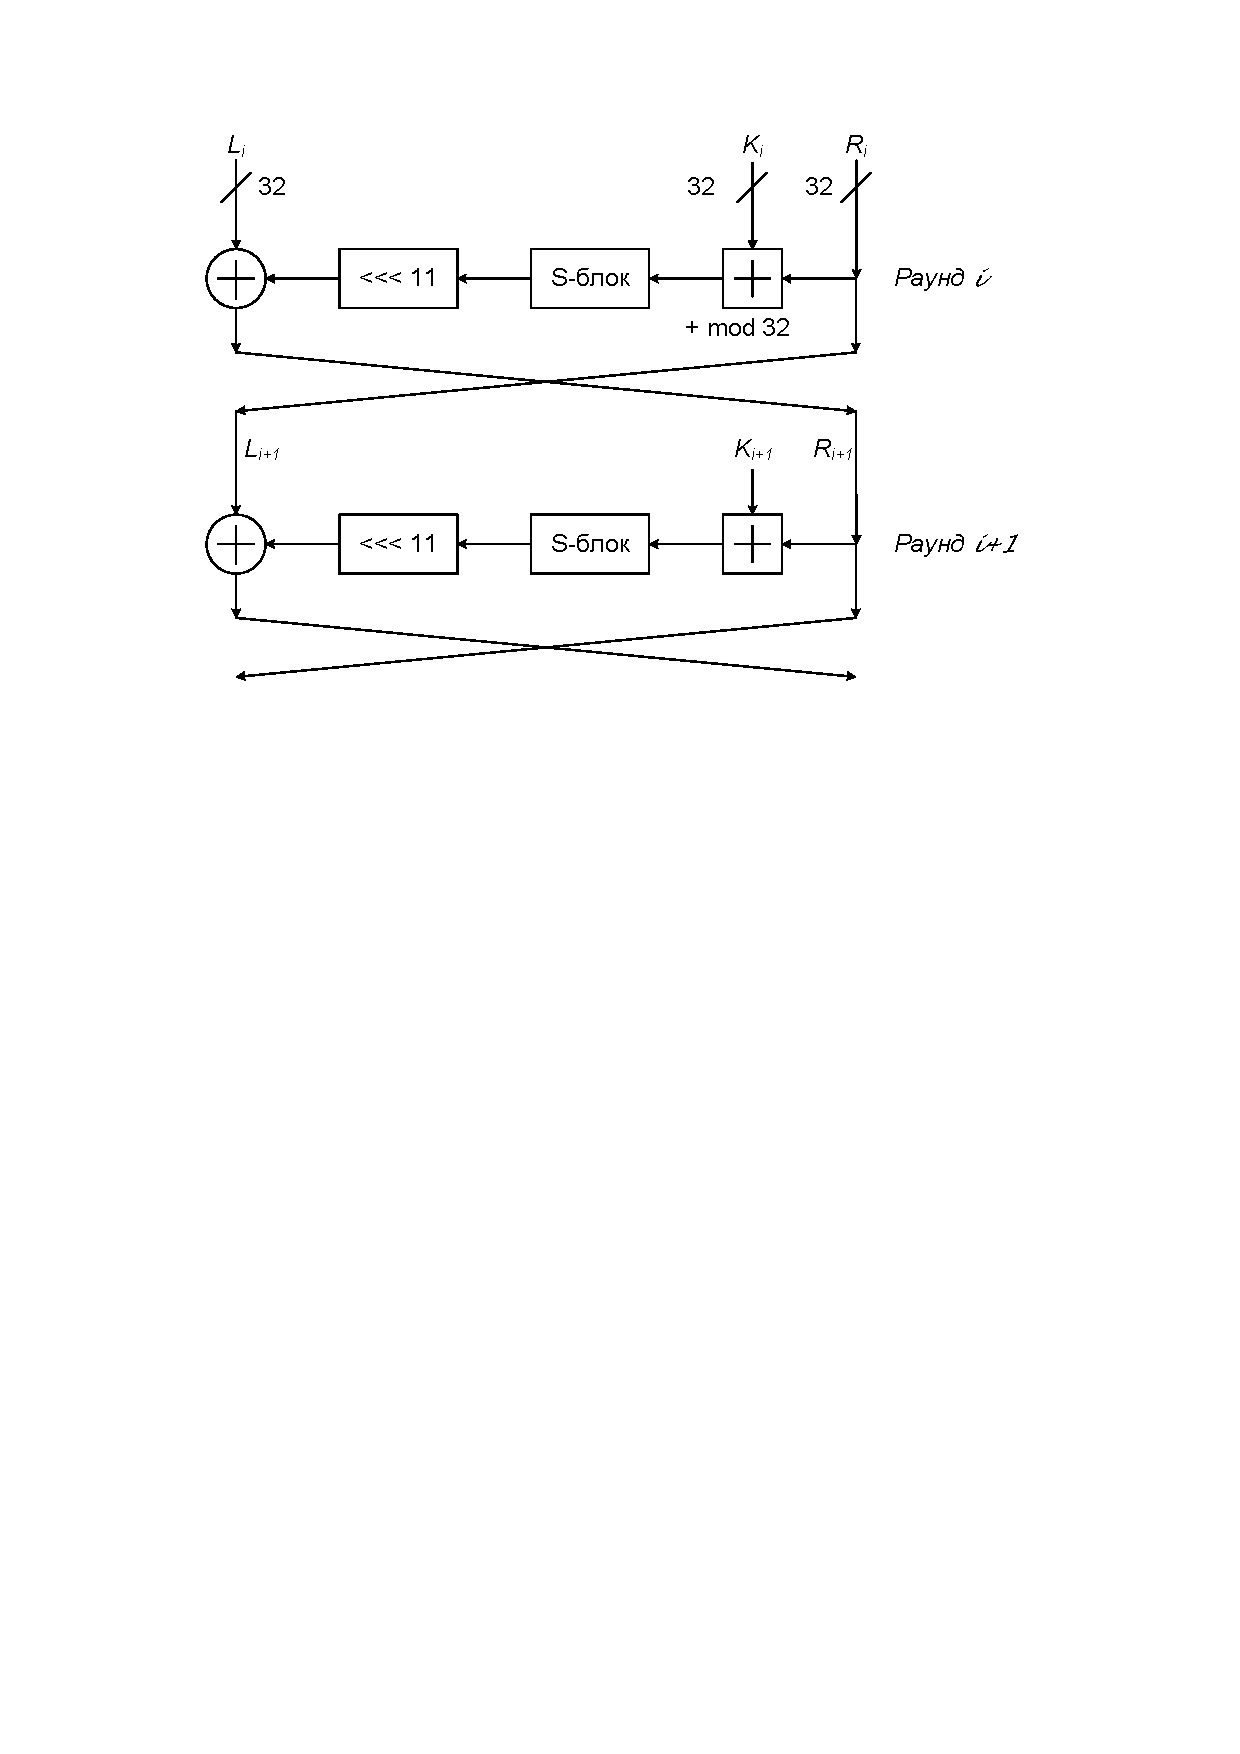
\includegraphics[width=0.6\textwidth]{pic/gost-28147-89}
    \caption{Схема ГОСТ 28147-89\label{fig:gost-28147-89}}
\end{figure}

Структурная схема алгоритма шифрования представлена на рисунке \ref{fig:gost-28147-89} и включает
\begin{itemize}
    \item ключевое запоминающее устройство (КЗУ) на 256 бит, которое состоит из восьми 32-разрядных накопителей $(X_0, X_1, X_2, X_3, X_4, X_5, X_6, X_7)$ и содержит сеансовые ключи шифрования одного раунда;
    \item 32-разрядный сумматор $\boxplus$ по модулю $2^{32}$;
    \item сумматор $\oplus$ по модулю 2;
    \item блок подстановки $(S)$;
    \item регистр циклического сдвига на одиннадцать шагов в сторону старшего разряда  $(R)$.
\end{itemize}

Блок подстановки $(S)$ состоит из 8 узлов замены, $s$-блоков, с памятью на 64 бита каждый. Поступающий на блок подстановки 32-разрядный вектор разбивается на восемь последовательных 4-разрядных векторов, каждый из которых преобразуется в 4-разрядный вектор соответствующим узлом замены. Узел замены представляет собой таблицу из шестнадцати строк, содержащих по четыре бита в строке. Входной вектор определяет адрес строки в таблице, заполнение данной строки является выходным вектором. Затем 4-разрядные выходные векторы последовательно объединяются в 32-разрядный вектор.

При перезаписи информации содержимое $i$-го разряда одного накопителя переписывается в $i$-й разряд другого накопителя.

Ключ, определяющий заполнение КЗУ, и таблицы блока подстановки $K$ являются секретными элементами.

Стандарт не накладывает ограничений на степень секретности защищаемой информации.

ГОСТ 28147-89 удобен как для аппаратной, так и для программной реализации.

Алгоритм имеет четыре режима работы. Из них первые три режима шифрования и последний -- генерирования имитовставки (другие названия: инициализирующий вектор, синхропосылка).
\begin{itemize}
    \item простой замены;
    \item гаммирования;
    \item гаммирования с обратной связью;
    \item выработки имитовставки.
\end{itemize}


Подробно, данные режимы описаны в следующем разделе.
